%%%%%%%%%%%%%%%%%%%%%%%%%%%%%%%%%%%%%%%%%
% Beamer Presentation
% LaTeX Template
% Version 1.0 (10/11/12)
%
% This template has been downloaded from:
% http://www.LaTeXTemplates.com
%
% License:
% CC BY-NC-SA 3.0 (http://creativecommons.org/licenses/by-nc-sa/3.0/)
%
%%%%%%%%%%%%%%%%%%%%%%%%%%%%%%%%%%%%%%%%%

%----------------------------------------------------------------------------------------
%	PACKAGES AND THEMES
%----------------------------------------------------------------------------------------

\documentclass{beamer}

\mode<presentation> {

%\usetheme{default}
%\usetheme{Antibes}
%\usetheme{Boadilla}
%\usetheme{JuanLesPins}
\usetheme{Madrid}
%\usetheme{Rochester}



% As well as themes, the Beamer class has a number of color themes
% for any slide theme. Uncomment each of these in turn to see how it
% changes the colors of your current slide theme.

%\usecolortheme{beaver}
%\usecolortheme{dolphin}
%\usecolortheme{orchid}
%\usecolortheme{rose}
%\usecolortheme{seagull}
%\usecolortheme{seahorse}
%\usecolortheme{whale}
%\usecolortheme{wolverine}

%\setbeamertemplate{footline} % To remove the footer line in all slides uncomment this line
%\setbeamertemplate{footline}[page number] % To replace the footer line in all slides with a simple slide count uncomment this line

%\setbeamertemplate{navigation symbols}{} % To remove the navigation symbols from the bottom of all slides uncomment this line

\setbeamertemplate{caption}[numbered]
}

\usepackage{graphicx}
\usepackage{booktabs}
\usepackage[%
	autocite    = superscript,
	backend     = bibtex,
	sortcites   = true,
	style       = numeric,
]{biblatex}
\addbibresource{reference.bib}

%----------------------------------------------------------------------------------------
%	TITLE PAGE
%----------------------------------------------------------------------------------------

\title[High speed Flight]{Learning High-Speed Flight in the Wild \autocite{high-speed-flight}}
\author{Edwin Jose George}
\institute[GCEK]{
	Guided by Dr. Rafeeque P C \\
	\medskip
	Department of Computer Science and Engineering \\
	Government College of Engineering Kannur
}
\date{\today}

\begin{document}

\begin{frame}
	\titlepage
\end{frame}

\begin{frame}{Overview}
	\tableofcontents
\end{frame}

%----------------------------------------------------------------------------------------
%	PRESENTATION SLIDES
%----------------------------------------------------------------------------------------
\section{Introduction}
\begin{frame}{Quad-drones}
	\begin{itemize}
		\item They are the most agile and dynamic machines, traversing extremely complex environments at high speeds. 
		\item This ability has led to their application in fields such as search and rescue, logistics, security, infrastructure, entertainment, and agriculture.
		\item To date, only expert human pilots have been able to fully exploit their capabilities. 
		\item Training of expert piolts - time consuming and costly
		\item The limiting factor for autonomous agile flight in arbitrary unknown environments is the coupling of fast and robust perception with effective planning. 
	\end{itemize}
\end{frame}

\begin{frame}{State of the art}
	\begin{itemize}
		\item Autonomous operation with onboard sensing and computation has been limited to low speeds. 
		\item Separate the navigation problem into subtasks: sensing, mapping, and planning. \\
		This approach has proven successful at low speeds
		\item The sub tasks are executed sequentially, leading to increased processing latency and compounding of errors through the pipeline.
		\item These issues can be mitigated to some degree by careful hand-tuning and engineering.
	\end{itemize}
\end{frame}

\begin{frame}{Proposed Solution}
	\begin{itemize}
		\item Here we propose an end-to-end approach that can autonomously fly quad rotors through complex natural and human-made environments at high speeds, with purely onboard sensing and computation.
		
		\item The key principle is to directly map noisy sensory observations to collision-free trajectories in a receding-horizon \autocite{receding_horizon} fashion. 
		
		\item This direct mapping drastically reduces processing latency and increases robustness to noisy and incomplete perception. 
		
		\item The sensorimotor mapping is performed by a convolutional network
	\end{itemize}
\end{frame}

\begin{frame}{Constraints to meet}
	\begin{itemize}
		\item The perception system has to be robust to disturbances such as sensor noise, motion blur, and changing illumination conditions
		\item An effective planner is necessary to find a path that is both dynamically feasible and collision-free while relying only on noisy and partial observations of the environment.
		\item The limited computational resources that are available on board, make it difficult to achieve reliable perception and effective planning at low latency and high speeds.
		\item Other factors such as aerodynamics, torque, power, reaction delays etc.
	\end{itemize}
	The limiting factor for autonomous agile flight in arbitrary unknown environments is the \textbf{\textit{coupling of fast and robust perception with effective planning}}.
\end{frame}

\begin{frame}{Training}
	\begin{itemize}
		\item Trained exclusively in simulation via privileged learning: imitating an expert with access to privileged information. 
		\item By simulating realistic sensor noise, this approach achieves zero-shot transfer from simulation to challenging real-world environments that were never experienced during training.		
	\end{itemize}
\end{frame}

\begin{frame}{Results}
	End-to-end policies trained in simulation enable high-speed autonomous flight through challenging environments, outperforming traditional obstacle avoidance pipelines.
\end{frame}

\begin{frame}{State of the art Model}
	\begin{itemize}
		\item Some works tackle only perception and build high-quality maps from imperfect measurements [5–9], 
		\item Other works focus on planning without considering perception errors [10–13]. 
		\item Numerous systems that combine online mapping with traditional planning algorithms have been proposed to achieve autonomous flight in previously unknown environments [14–22]. 
	\end{itemize}
\end{frame}

\begin{frame}{Taxonomy of existing approaches for drone navigation}
	\centering
	\begin{figure}
		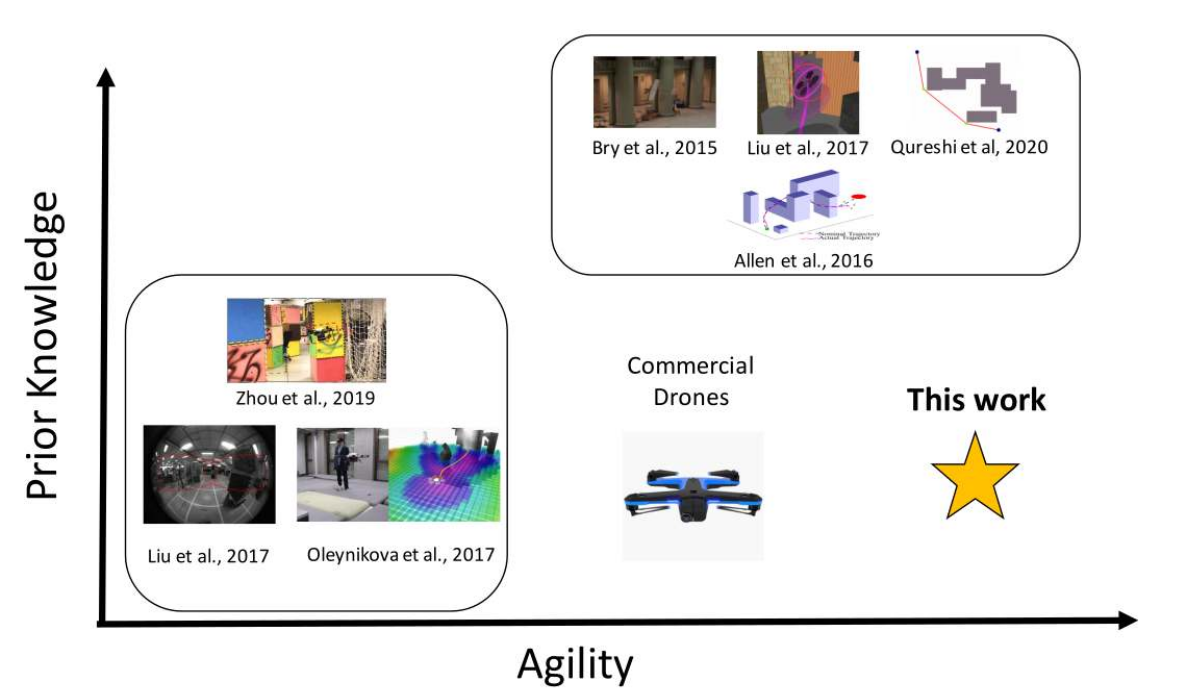
\includegraphics[height=2in]{images/taxonomy_navigation.png}
		\caption{Taxonomy of existing approaches for drone navigation in challenging and cluttered environments. Approaches are ordered with
respect to the required prior knowledge about the environment and the maximum agility they achieve.}
	\end{figure}
\end{frame}

\begin{frame}{Traditional Method}
	The division of the navigation task into the \textbf{mapping and planning subtasks} is 
	\begin{itemize}
		\item Attractive from an engineering perspective because it enables parallel progress on each component and makes the overall system interpretable. 
		\item It leads to pipelines that largely neglect interactions between the different stages and thus compound errors. 
		\item Their sequential nature also introduces additional latency.
	\end{itemize}
\end{frame}

\begin{frame}{Recent works}
	\begin{itemize}
		\item Propose to learn end-to-end policies directly from data without explicit mapping and planning stages. 
		\item These policies are trained by imitating a human, from experience that was collected in simulation, or directly in the real world. More recent work has demonstrated that very agile control policies can be trained in simulation. 
		\item Policies produced by the last approach can successfully perform acrobatic maneuvers, but can only operate in unobstructed free space and are essentially blind to obstacles in the environment.
	\end{itemize}
\end{frame}

\begin{frame}{This works}
	Here we present an approach to fly a quad rotor at high speeds in a variety of environments with complex obstacle geometry while having access to only onboard sensing and computation. By predicting navigation commands directly from sensor measurements, we decrease the latency between perception and action while simultaneously being robust to perception artifacts, such as motion blur, missing data, and sensor noise.
\end{frame}

\begin{frame}{Input}
	We leverage the abstraction of the input data to transfer the policy from simulation to reality. To this end, we utilize a stereo matching algorithm \autocite{stereoMatching} to provide depth images as input to the policy. 
\end{frame}


\begin{frame}{Navigation Policy}
	We train the navigation policy via privileged learning \autocite{Privileged_Learning} on demonstrations that are provided by a sampling-based expert. The existing global planning algorithms \autocite{global_planning} generally output a single trajectory, our expert uses Metropolis-Hastings \autocite{MH_hasting} sampling to compute a distribution of collision-free trajectories. We use our planner to compute trajectories with a short time horizon to ensure that they are predictable from onboard sensors and that the sampler remains computationally tractable. We bias the sampler toward obstacle-free regions by conditioning it on trajectories from a classic global planning algorithm [13].
	
\end{frame}

\begin{frame}{Neural Network Policy}
	We also reflect the multi-modal nature of the problem in the design and training of the neural network policy. Our policy takes a noisy depth image and inertial measurements as sensory inputs and produces a set of short-term trajectories together with an estimate of individual trajectory costs. The trajectories are represented as high-order polynomials to ensure dynamical feasibility. We train the policy using a multi-hypothesis winner-takes-all loss that adaptively maps the predicted trajectories to the best trajectories that have been found by the sampling-based expert. The policy network is designed to be extremely lightweight, which ensures that it can be executed on board the quadrotor at the update rates required for high-speed flight.
	
\end{frame}


\section{References}
\begin{frame}[allowframebreaks, noframenumbering]{References}
	\printbibliography
\end{frame}

%------------------------------------------------
\section{First Section}
%------------------------------------------------

\subsection{Subsection Example} % A subsection can be created just before a set of slides with a common theme to further break down your presentation into chunks

\begin{frame}
\frametitle{Paragraphs of Text}
Sed iaculis dapibus gravida. Morbi sed tortor erat, nec interdum arcu. Sed id lorem lectus. Quisque viverra augue id sem ornare non aliquam nibh tristique. Aenean in ligula nisl. Nulla sed tellus ipsum. Donec vestibulum ligula non lorem vulputate fermentum accumsan neque mollis.\\~\\

Sed diam enim, sagittis nec condimentum sit amet, ullamcorper sit amet libero. Aliquam vel dui orci, a porta odio. Nullam id suscipit ipsum. Aenean lobortis commodo sem, ut commodo leo gravida vitae. Pellentesque vehicula ante iaculis arcu pretium rutrum eget sit amet purus. Integer ornare nulla quis neque ultrices lobortis. Vestibulum ultrices tincidunt libero, quis commodo erat ullamcorper id.
\end{frame}

%------------------------------------------------

\begin{frame}
\frametitle{Bullet Points}
\begin{itemize}
\item Lorem ipsum dolor sit amet, consectetur adipiscing elit
\item Aliquam blandit faucibus nisi, sit amet dapibus enim tempus eu
\item Nulla commodo, erat quis gravida posuere, elit lacus lobortis est, quis porttitor odio mauris at libero
\item Nam cursus est eget velit posuere pellentesque
\item Vestibulum faucibus velit a augue condimentum quis convallis nulla gravida
\end{itemize}
\end{frame}

%------------------------------------------------

\begin{frame}
\frametitle{Blocks of Highlighted Text}
\begin{block}{Block 1}
Lorem ipsum dolor sit amet, consectetur adipiscing elit. Integer lectus nisl, ultricies in feugiat rutrum, porttitor sit amet augue. Aliquam ut tortor mauris. Sed volutpat ante purus, quis accumsan dolor.
\end{block}

\begin{block}{Block 2}
Pellentesque sed tellus purus. Class aptent taciti sociosqu ad litora torquent per conubia nostra, per inceptos himenaeos. Vestibulum quis magna at risus dictum tempor eu vitae velit.
\end{block}

\begin{block}{Block 3}
Suspendisse tincidunt sagittis gravida. Curabitur condimentum, enim sed venenatis rutrum, ipsum neque consectetur orci, sed blandit justo nisi ac lacus.
\end{block}
\end{frame}

%------------------------------------------------

\begin{frame}
\frametitle{Multiple Columns}
\begin{columns}[c] % The "c" option specifies centered vertical alignment while the "t" option is used for top vertical alignment

\column{.45\textwidth} % Left column and width
\textbf{Heading}
\begin{enumerate}
\item Statement
\item Explanation
\item Example
\end{enumerate}

\column{.5\textwidth} % Right column and width
Lorem ipsum dolor sit amet, consectetur adipiscing elit. Integer lectus nisl, ultricies in feugiat rutrum, porttitor sit amet augue. Aliquam ut tortor mauris. Sed volutpat ante purus, quis accumsan dolor.

\end{columns}
\end{frame}

%------------------------------------------------
\section{Second Section}
%------------------------------------------------

\begin{frame}
\frametitle{Table}
\begin{table}
\begin{tabular}{l l l}
\toprule
\textbf{Treatments} & \textbf{Response 1} & \textbf{Response 2}\\
\midrule
Treatment 1 & 0.0003262 & 0.562 \\
Treatment 2 & 0.0015681 & 0.910 \\
Treatment 3 & 0.0009271 & 0.296 \\
\bottomrule
\end{tabular}
\caption{Table caption}
\end{table}
\end{frame}

%------------------------------------------------

\begin{frame}
\frametitle{Theorem}
\begin{theorem}[Mass--energy equivalence]
$E = mc^2$
\end{theorem}
\end{frame}

%------------------------------------------------

\begin{frame}[fragile] % Need to use the fragile option when verbatim is used in the slide
\frametitle{Verbatim}
\begin{example}[Theorem Slide Code]
\begin{verbatim}
\begin{frame}
\frametitle{Theorem}
\begin{theorem}[Mass--energy equivalence]
$E = mc^2$
\end{theorem}
\end{frame}\end{verbatim}
\end{example}
\end{frame}

%------------------------------------------------

\begin{frame}
\frametitle{Figure}
Uncomment the code on this slide to include your own image from the same directory as the template .TeX file.
%\begin{figure}
%\includegraphics[width=0.8\linewidth]{test}
%\end{figure}
\end{frame}

%------------------------------------------------

\begin{frame}[fragile] % Need to use the fragile option when verbatim is used in the slide
\frametitle{Citation}
An example of the \verb|\cite| command to cite within the presentation:\\~

This statement requires citation.
\end{frame}

%------------------------------------------------

\begin{frame}
\frametitle{References}
\footnotesize{
\begin{thebibliography}{99} % Beamer does not support BibTeX so references must be inserted manually as below
\bibitem[Smith, 2012]{p1} John Smith (2012)
\newblock Title of the publication
\newblock \emph{Journal Name} 12(3), 45 -- 678.
\end{thebibliography}
}
\end{frame}

%------------------------------------------------

\begin{frame}
\Huge{\centerline{The End}}
\end{frame}

%----------------------------------------------------------------------------------------

\end{document} 